\begin{figure}[H]
    \center
    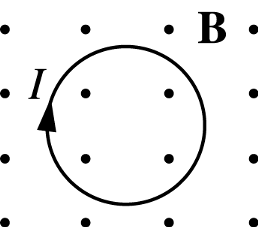
\includegraphics[scale=0.25]{images/img-010-019.png}
\end{figure}

% Multiple Choice Question 27
\begin{questions}\setcounter{question}{26}\question
A loop of wire carrying a steady current $I$ is initially at rest perpendicular to a uniform magnetic field of magnitude $B$, as shown above. The loop is then rotated about a diameter at a constant rate. The torque on the loop is maximum when the loop has rotated, with respect to its initial position, through an angle of

\begin{oneparchoices}
\choice $30^{\circ}$
\choice $45^{\circ}$
\choice $90^{\circ}$
\choice $180^{\circ}$
\choice $360^{\circ}$
\end{oneparchoices}\end{questions}

